\section{广度优先遍历}
\label{sec:graph-bfs}

从一个起点出发，哪些顶点能够到达，到达每个顶点最少要走几条边，又该沿哪条路线走？按定义逐条检查路径行不通，因为路径数目可能极多。一个更经济的想法是按距离分层推进：先找出起点的全部邻居，它们离起点一条边；再找出这些邻居的尚未见过的邻居，它们离起点两条边；如此继续，直到没有新顶点出现。本节把这个想法写成算法，说明队列怎样保证“先近后远”，并证明算法记录的层数确实是最少边数。

\subsection{广度优先遍历算法}
\label{sec:graph-trav-bfs-algorithm}

\paragraph{需要记录的状态}
按层推进时，要知道哪些顶点已经见过、哪些顶点等待展开、每个顶点在第几层、它是从哪个顶点过来的。于是对起点$s$维护四项状态：发现标记，表示顶点是否已经被找到；一个先进先出的队列$Q$，存放已经发现、但邻居尚未检查的顶点；边数距离$d(v)$；以及\term{父指针}（parent pointer）$p(v)$，记录$v$是从哪个顶点第一次被找到的。初始时只有$s$被发现，$d(s)=0$，$p(s)$为空，队列为$[s]$；其余顶点未发现，距离记为$+\infty$。这种按层访问的过程称为广度优先遍历，也常称\term{广度优先搜索}（breadth-first search，BFS）。

\begin{algorithm}[广度优先遍历]
\label{alg:graph-trav-bfs}
输入：图$\mathcal G=(V,E)$的邻接表，起点$s\in V$。输出：距离$d(v)$与父指针$p(v)$，$v\in V$。
\begin{enumerate}
  \item 标记$s$为已发现，置$d(s)=0$、$p(s)$为空，令$Q=[s]$；其余顶点未发现，$d(v)=+\infty$。
  \item 当$Q$非空时，取出队首$u$，按邻接表依次读取$u$的邻居$v$（有向图只读出邻居$v\in N^+(u)$）。若$v$未发现，立即标记$v$为已发现，置$d(v)=d(u)+1$、$p(v)=u$，并把$v$放到队尾；若$v$已发现，跳过。
  \item 队列为空时停止。
\end{enumerate}
\end{algorithm}

标记必须在入队时完成，而不是等到出队时。两个已发现的顶点可能共享一个尚未发现的邻居；若出队时才标记，这个邻居会被两个顶点各放入队列一次，距离和父指针也可能被改写。入队即标记保证每个顶点至多入队一次。

\paragraph{贯穿图上的队列轨迹}
在第~\ref{sec:graph-basic-concepts}节的贯穿四点图上，以$1$为起点，并约定按编号从小到大读取邻居。图~\ref{fig:graph-trav-bfs-queue}(b)逐行列出了每次出队后的队列。取出$1$时发现$2,3$，队列变为$[2,3]$；取出$2$时，邻居$1,3$都已发现，只有$4$是新的，队列变为$[3,4]$；取出$3$时，邻居$1,2,4$全部已发现，$4$不会第二次入队；最后取出$4$，队列为空。结果是$d(2)=d(3)=1$、$d(4)=2$，父指针为$p(2)=p(3)=1$、$p(4)=2$。图~\ref{fig:graph-trav-bfs-queue}(a)把各顶点按$d$值分到三层，蓝色箭头就是父指针所指的边。

\begin{figure}[!htb]
  \centering
  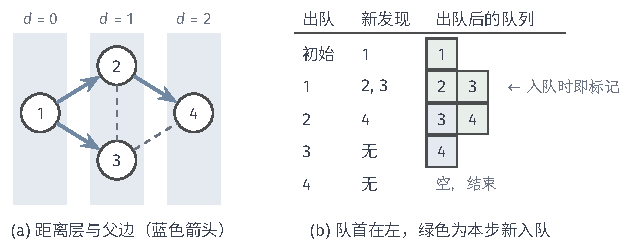
\includegraphics[width=106.7mm]{figures/01-basic-mathematics/04-graphs/tikz/c2-bfs-queue-trace/figure.pdf}
  \caption{贯穿四点图上从顶点$1$出发的广度优先遍历，邻居按编号递增读取。(a)顶点按边数距离$d$分为三层，蓝色箭头是父指针对应的边，虚线是检查过但没有带来新顶点的边。(b)每次出队后的队列，队首在左，绿色格子是这一步新入队的顶点；取出$3$时$4$已在队中，不再重复入队。}
  \label{fig:graph-trav-bfs-queue}
\end{figure}

\paragraph{由父指针恢复路线}
父指针给出的是一条实际路线，而不只是一个距离数值。要得到从$s$到已发现顶点$t$的路线，从$t$出发反复取父指针，直到回到$s$，再把得到的顶点序列反转。在上例中，$4$的父指针是$2$，$2$的父指针是$1$，反转后得到路线$1\to2\to4$，恰有$d(4)=2$条边。父指针总是指向更早发现的顶点，所以沿父指针回溯不会绕圈，一定在有限步内回到$s$。若$t$始终未被发现，即$d(t)=+\infty$，算法应报告$t$从$s$不可达，而不能输出任何路线。

路线并不唯一。若把邻居的读取次序改为先读$3$再读$2$，那么取出$1$后队列为$[3,2]$，$4$会在展开$3$时被发现，父指针变成$p(4)=3$，路线变成$1\to3\to4$。两条路线不同，但边数都是$2$。下面的定理说明，改变同层顶点的处理次序可能改变父指针，却不会改变距离。

\subsection{正确性与计算开销}
\label{sec:graph-trav-bfs-correctness}

\paragraph{为什么首次记录就是最少边数}
记$\operatorname{dist}(s,v)$为从$s$到$v$的路径的最少边数，不可达时为$+\infty$。算法只在顶点第一次被发现时写入$d(v)$，以后不再修改。我们要说明，这个“第一次”恰好发生在最短的距离上。

\begin{theorem}[广度优先遍历的距离]
\label{thm:graph-trav-bfs-distance}
设对有限图$\mathcal G$和起点$s$执行算法~\ref{alg:graph-trav-bfs}。则对每个顶点$v$，$d(v)=\operatorname{dist}(s,v)$；当$v$可达时，沿父指针从$v$回到$s$的路线恰有$d(v)$条边。
\end{theorem}

\begin{proof}
先说明$d(v)$不会小于真实距离。若$d(v)$有限且$v\neq s$，则$d(p(v))=d(v)-1$，沿父指针每退一步距离减一，$d(v)$步后回到$s$。反转这串顶点就得到一条从$s$到$v$、恰有$d(v)$条边的路线，所以$d(v)\geq\operatorname{dist}(s,v)$。

再说明队列中的距离值有一个固定的形状：从队首到队尾不减，且最大值与最小值至多相差$1$。初始队列只有$s$，满足这一点。设某时刻队列中的值为若干个$k$后接若干个$k+1$，取出的队首$u$有$d(u)=k$，新加入的顶点距离都是$k+1$，并放在队尾，形状仍然保持。由此可知，顶点出队时的距离值按时间不减。

最后对$\delta=\operatorname{dist}(s,v)$归纳，证明有限距离的顶点都会被发现且$d(v)\leq\delta$。$\delta=0$时$v=s$。设$\delta\geq1$，并设距离小于$\delta$的顶点都已满足结论。取一条从$s$到$v$的最短路径，记其倒数第二个顶点为$x$，则$\operatorname{dist}(s,x)=\delta-1$，由归纳假设$x$被发现且$d(x)=\delta-1$。$x$入过队，就一定在某一时刻出队并检查邻居$v$。若此时$v$尚未发现，就得到$d(v)=d(x)+1=\delta$；若$v$已经被发现，则发现它的顶点$u$出队不晚于$x$，按上一段的单调性$d(u)\leq d(x)$，于是$d(v)=d(u)+1\leq\delta$。两个方向合起来得到$d(v)=\operatorname{dist}(s,v)$。不可达的顶点没有任何从$s$出发的路线，第一段说明它不可能得到有限的$d$值。
\end{proof}

证明的关键是第二段的队列形状：算法处理第$k$层时，只会首次发现第$k+1$层的顶点；第$k+1$层的顶点全部排在第$k$层之后。倒数第二个顶点$x$比$v$少一层，一定先被展开，因此$v$不可能等到更远的层才被发现。

\paragraph{计算开销}
以邻接表存储时，每个顶点至多入队一次、出队一次；每个顶点出队时把它的邻接表读一遍，因此每条邻接记录只被检查常数次。无向图的邻接记录共$2m$条，有向图的出邻接记录共$m$条，所以总时间为$O(n+m)$。发现标记、距离、父指针和队列各占$O(n)$额外空间。这一结论依赖“列出邻居的代价与度数成正比”。若图以邻接矩阵存储，找出一个顶点的邻居要扫描矩阵的一整行，$n$个顶点共扫描$n^2$个位置，时间变为$O(n^2)$；对稀疏图，这比$O(n+m)$大得多。

\paragraph{最少边数不是最小总长度}
广度优先遍历把每条边都算作一步。边上带有长度时，边数最少的路线不一定总长度最小。图~\ref{fig:graph-trav-bfs-weighted}中，从$s$直接到$t$只需一条边，广度优先遍历就会用这条边记录$t$，但它的长度是$5$；经过$a$的路线多走一条边，总长度却只有$1+1=2$。所以广度优先遍历只解决所有边长相等时的最短路问题。一般边长下的最短路需要比较累计长度，留到第~\ref{sec:graph-shortest-paths}节。

\begin{figure}[!htb]
  \centering
  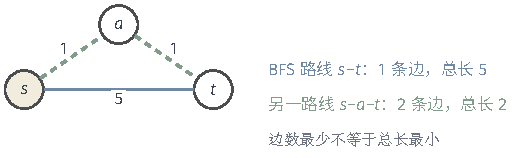
\includegraphics[width=87.8mm]{figures/01-basic-mathematics/04-graphs/tikz/c2-bfs-weighted-counterexample/figure.pdf}
  \caption{带权反例。边旁数字是长度。广度优先遍历从$s$出发时经直接边一步发现$t$（蓝色），这条路线总长$5$；绿色虚线路线$s\text{--}a\text{--}t$多一条边，总长只有$2$。广度优先遍历最小化的是边数，不是总长度。}
  \label{fig:graph-trav-bfs-weighted}
\end{figure}

此外，一次广度优先遍历只覆盖从$s$可达的部分。遍历结束时距离仍为$+\infty$的顶点没有被访问，不能据此断言它们是孤立点，它们之间可能有很多边。要给全图的每个顶点划分连通分量，需要在外层不断换新的起点重新启动，这是第~\ref{sec:graph-connectivity-computation}节的内容。

\subsection{多源广度优先遍历}
\label{sec:graph-trav-multi-source-bfs}

\paragraph{从一组起点同时出发}
有时关心的不是离某一个起点有多远，而是离一组起点中最近的那个有多远。例如在网格上放置若干个种子，问每个格子离最近的种子几步。给定起点集合$S\subseteq V$，定义
\[
\operatorname{dist}(S,v)=\min_{s\in S}\operatorname{dist}(s,v),
\]
空集上的最小值约定为$+\infty$。做法是把$S$中所有顶点同时作为第$0$层：初始时它们都被标记、距离为$0$、父指针为空，并按任意次序全部放入队列，此后完全按算法~\ref{alg:graph-trav-bfs}执行。这称为\term{多源广度优先遍历}（multi-source breadth-first search）。

为什么这样得到的是到最近起点的距离？设想添加一个新顶点$s^*$，从它向$S$中每个顶点连一条边（有向图中连弧$s^*\to s$）。在新图中，任一顶点$v\notin\{s^*\}$满足$\operatorname{dist}(s^*,v)=1+\operatorname{dist}(S,v)$，因为从$s^*$出发的路线第一步必然进入$S$中的某个点。从$s^*$做普通广度优先遍历，第一次出队就把$S$中所有顶点以距离$1$放入队列，此后的过程与多源版本完全相同，只是所有距离多了$1$。由定理~\ref{thm:graph-trav-bfs-distance}即得多源版本输出$\operatorname{dist}(S,v)$，而且沿父指针回溯会停在某个起点上，它就是离$v$最近的起点之一。

\paragraph{网格上的种子传播}
图~\ref{fig:graph-trav-multi-source}是一个$3\times5$网格，相邻格子以上下左右相连，中间一个格子不属于图。两个起点放在左上角和右下角，每个格子中的数字是它到较近起点的边数。例如第一行第四个格子离左上角$3$步、离右下角$3$步，记为$3$；第一行最右的格子离右下角只有$2$步，记为$2$。若只从左上角出发，右下角的格子距离为$6$。

\begin{figure}[!htb]
  \centering
  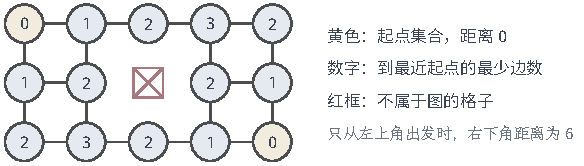
\includegraphics[width=99.0mm]{figures/01-basic-mathematics/04-graphs/tikz/c2-multi-source-bfs/figure.pdf}
  \caption{$3\times5$网格上的多源广度优先遍历。网格以上下左右相邻连边，红框格子不属于图；两个黄色起点同时作为第$0$层。每个顶点中的数字是到较近起点的最少边数，所有距离由一次遍历得到。}
  \label{fig:graph-trav-multi-source}
\end{figure}

\paragraph{与逐个起点遍历的区别}
多源遍历与“对每个起点各做一次广度优先遍历”回答的是不同问题。后者得到$|S|$组距离，能说出$v$到每一个起点各有多远，需要$O(|S|(n+m))$时间；多源遍历只给出到最近起点的距离及对应的起点，一次遍历只需$O(n+m)$时间。若$S$为空，队列一开始就为空，所有顶点保持未发现，输出的可达集为空集，这与$\operatorname{dist}(\varnothing,v)=+\infty$的约定一致。图像中从种子出发的区域生长是这一机制的典型用途；判断哪些像素属于前景、怎样选择邻接规则等完整处理留到应用部分。
